\documentclass{article}
\usepackage{graphicx}
\usepackage{amsmath}
\graphicspath{{./images}}

\title{CSCE 438: MP 2.1}
\author{Kevin Zhang}
\date{\today}

\begin{document}

\maketitle

\section{Overview}

In MP 2.1, our main goal is to develop a coordinator process that coordinates between clients and a \textit{group} of servers. To do so, we need a deterministic way for clients to be assigned to a specific server, and we need the servers to register themselves with the coordinator.

\section{Client-Coordinator Interaction}

When client processes start up, they immediately contact the coordinator process (whose host and port are known to the client) to get assigned to a cluster/server. The coordinator responds with the IP address and port of the client's assigned server.\\

\noindent The coordinator determine the client's assigned server with the following formula:

\[ clusterID = (clientID - 1)\ \%\ 3 + 1 \]
\[ serverID = \text{first server registered to } clusterID \]

\noindent Where \textit{clientID} is the same as the client's username. Here, we perform modulus by 3 because we assume a fixed number of clusters (3). Additionally, for this MP, we assume that each cluster only has up to one server, so we simply return the first server registered under each cluster.

\section{Client-Server Interaction}

For this MP, the client-server interaction remains largely the same. Once a client is assigned a server, they cannot change which server they are assigned to. Consequently, if the client's server goes down, they cannot access the SNS.\\

\noindent The only difference, which will not be explored in this MP, is that the method the server uses to update client posts is different.

\section{Coordinator-Server Interaction}

One of the primary jobs of the coordinator process is to register every server in its registration table. The coordinator will use this table to track the liveness status of each server and assign servers to clients.\\

\noindent For a server to register itself, it sends ``heartbeat'' messages periodically to the coordinator. Each message contains the server's cluster ID and a \texttt{ServerInfo} gRPC object containing the server's ID, hostname, port, and type (i.e. follower coordinator or server).\\

\noindent On the first heartbeat message the coordinator receives from a server, the coordinator adds the server to its list of registered servers. It now expects a heartbeat at least every 10 seconds for the server to remain ``alive.'' If 10 seconds elapse since a server sends a heartbeat, the coordinator declares the server ``dead.''

\newpage
\section{Test Cases}

\subsection{Test 1: Sanity check}

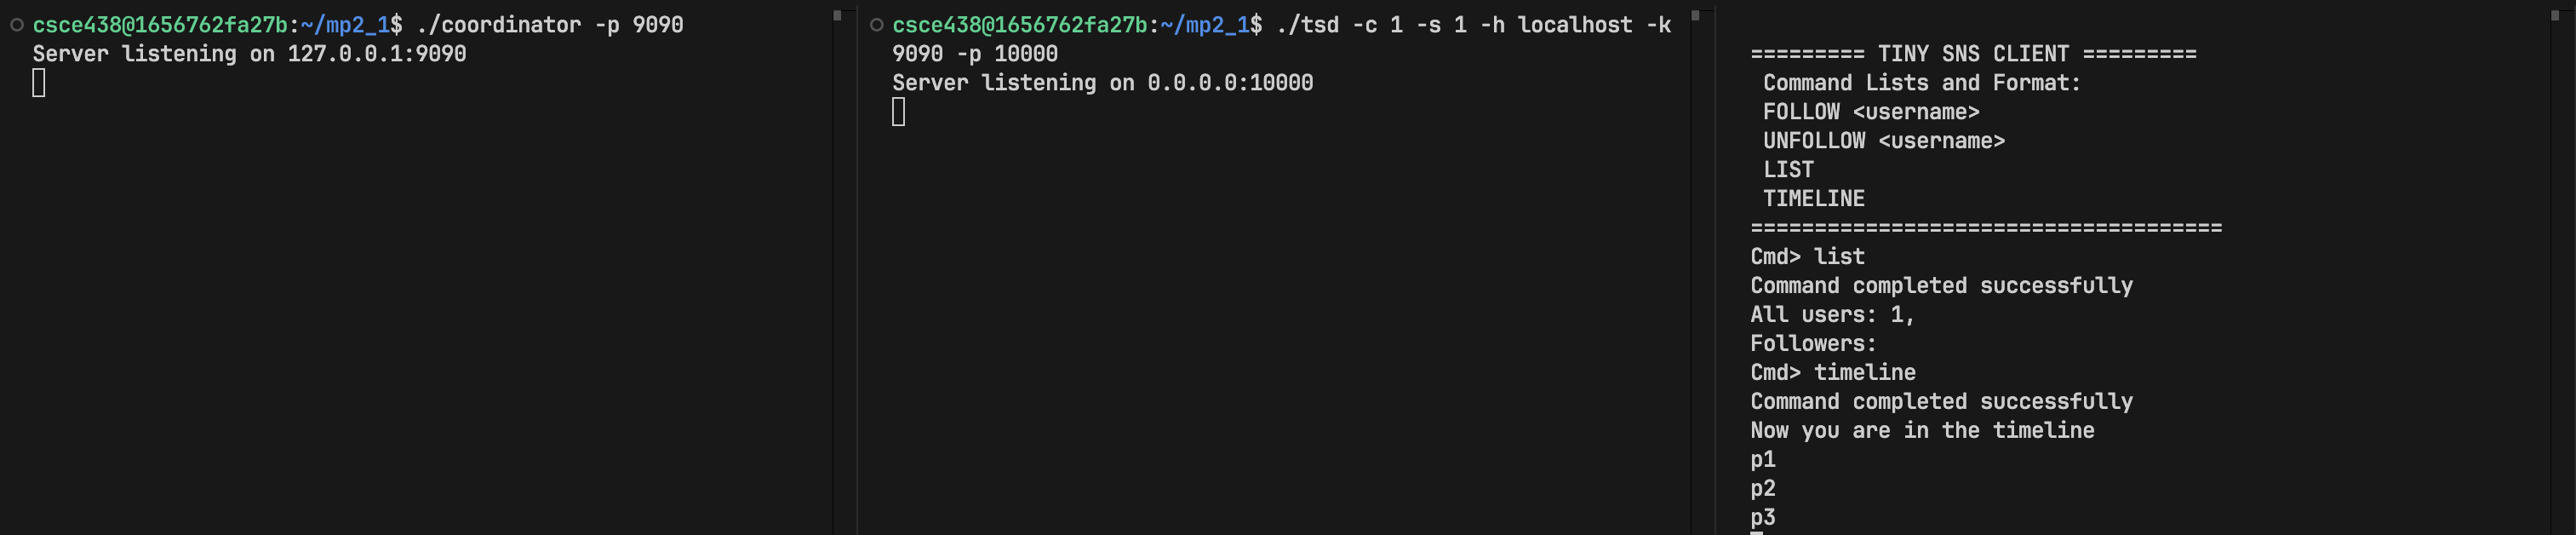
\includegraphics[width=\textwidth]{test1}

\subsection{Test 2: Kill server before client}

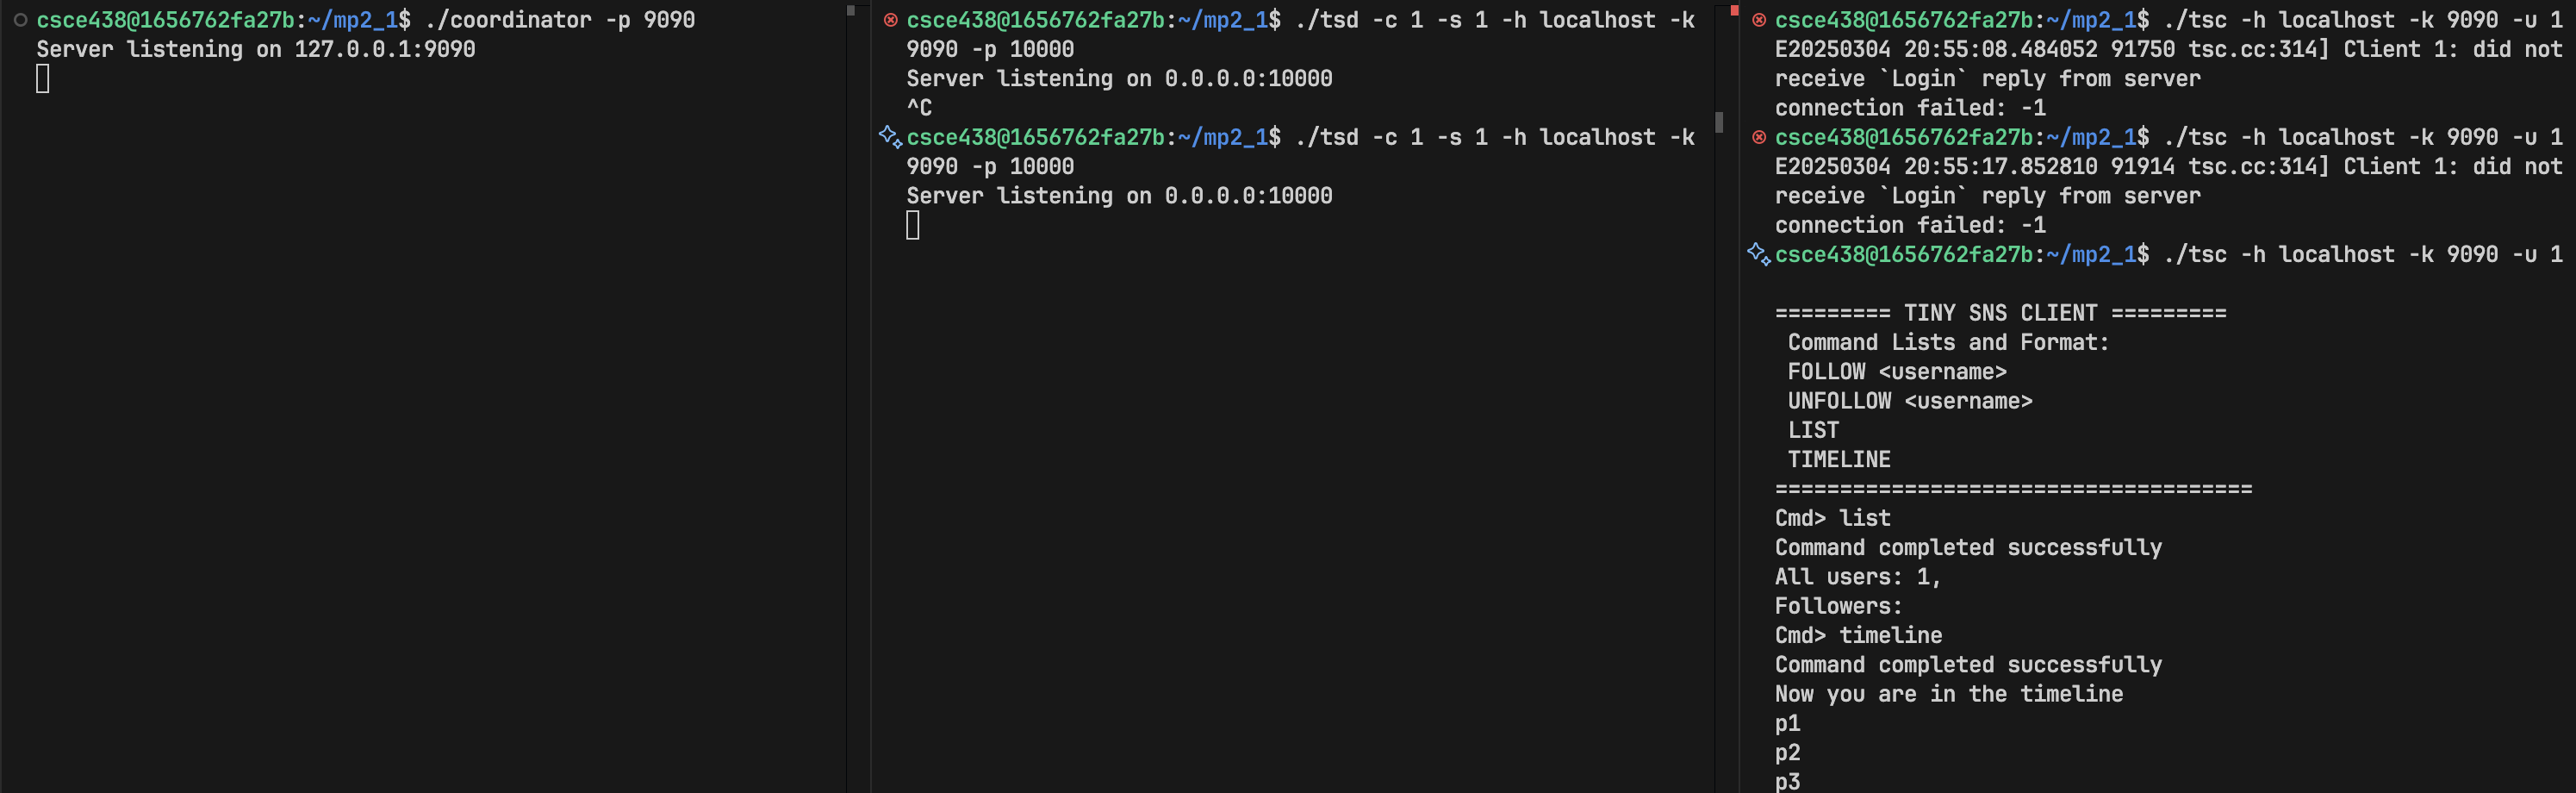
\includegraphics[width=\textwidth]{test2}

\subsection{Test 3: Kill server after client}

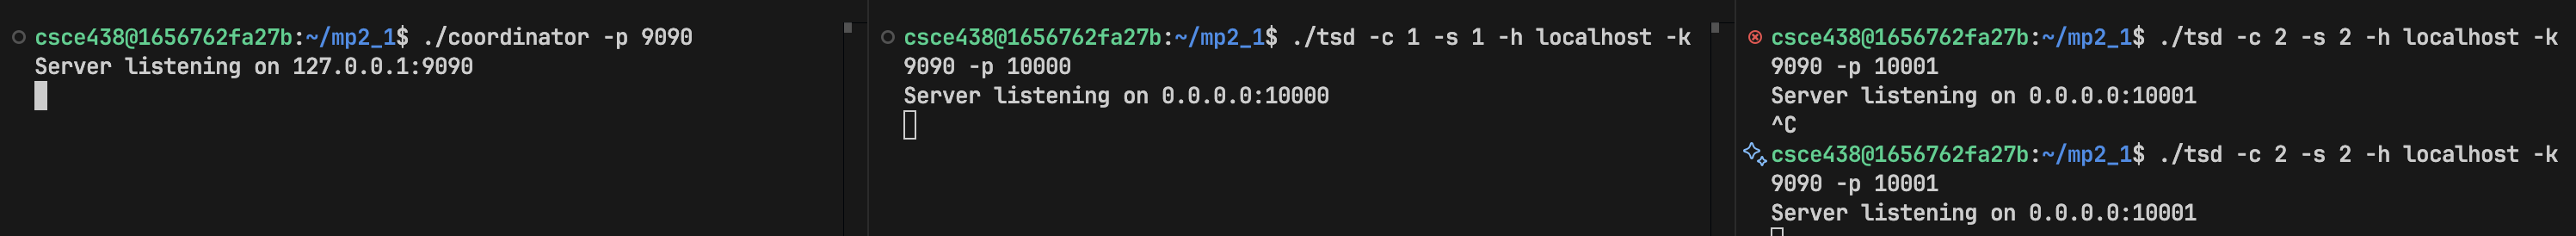
\includegraphics[width=\textwidth]{test3-1}
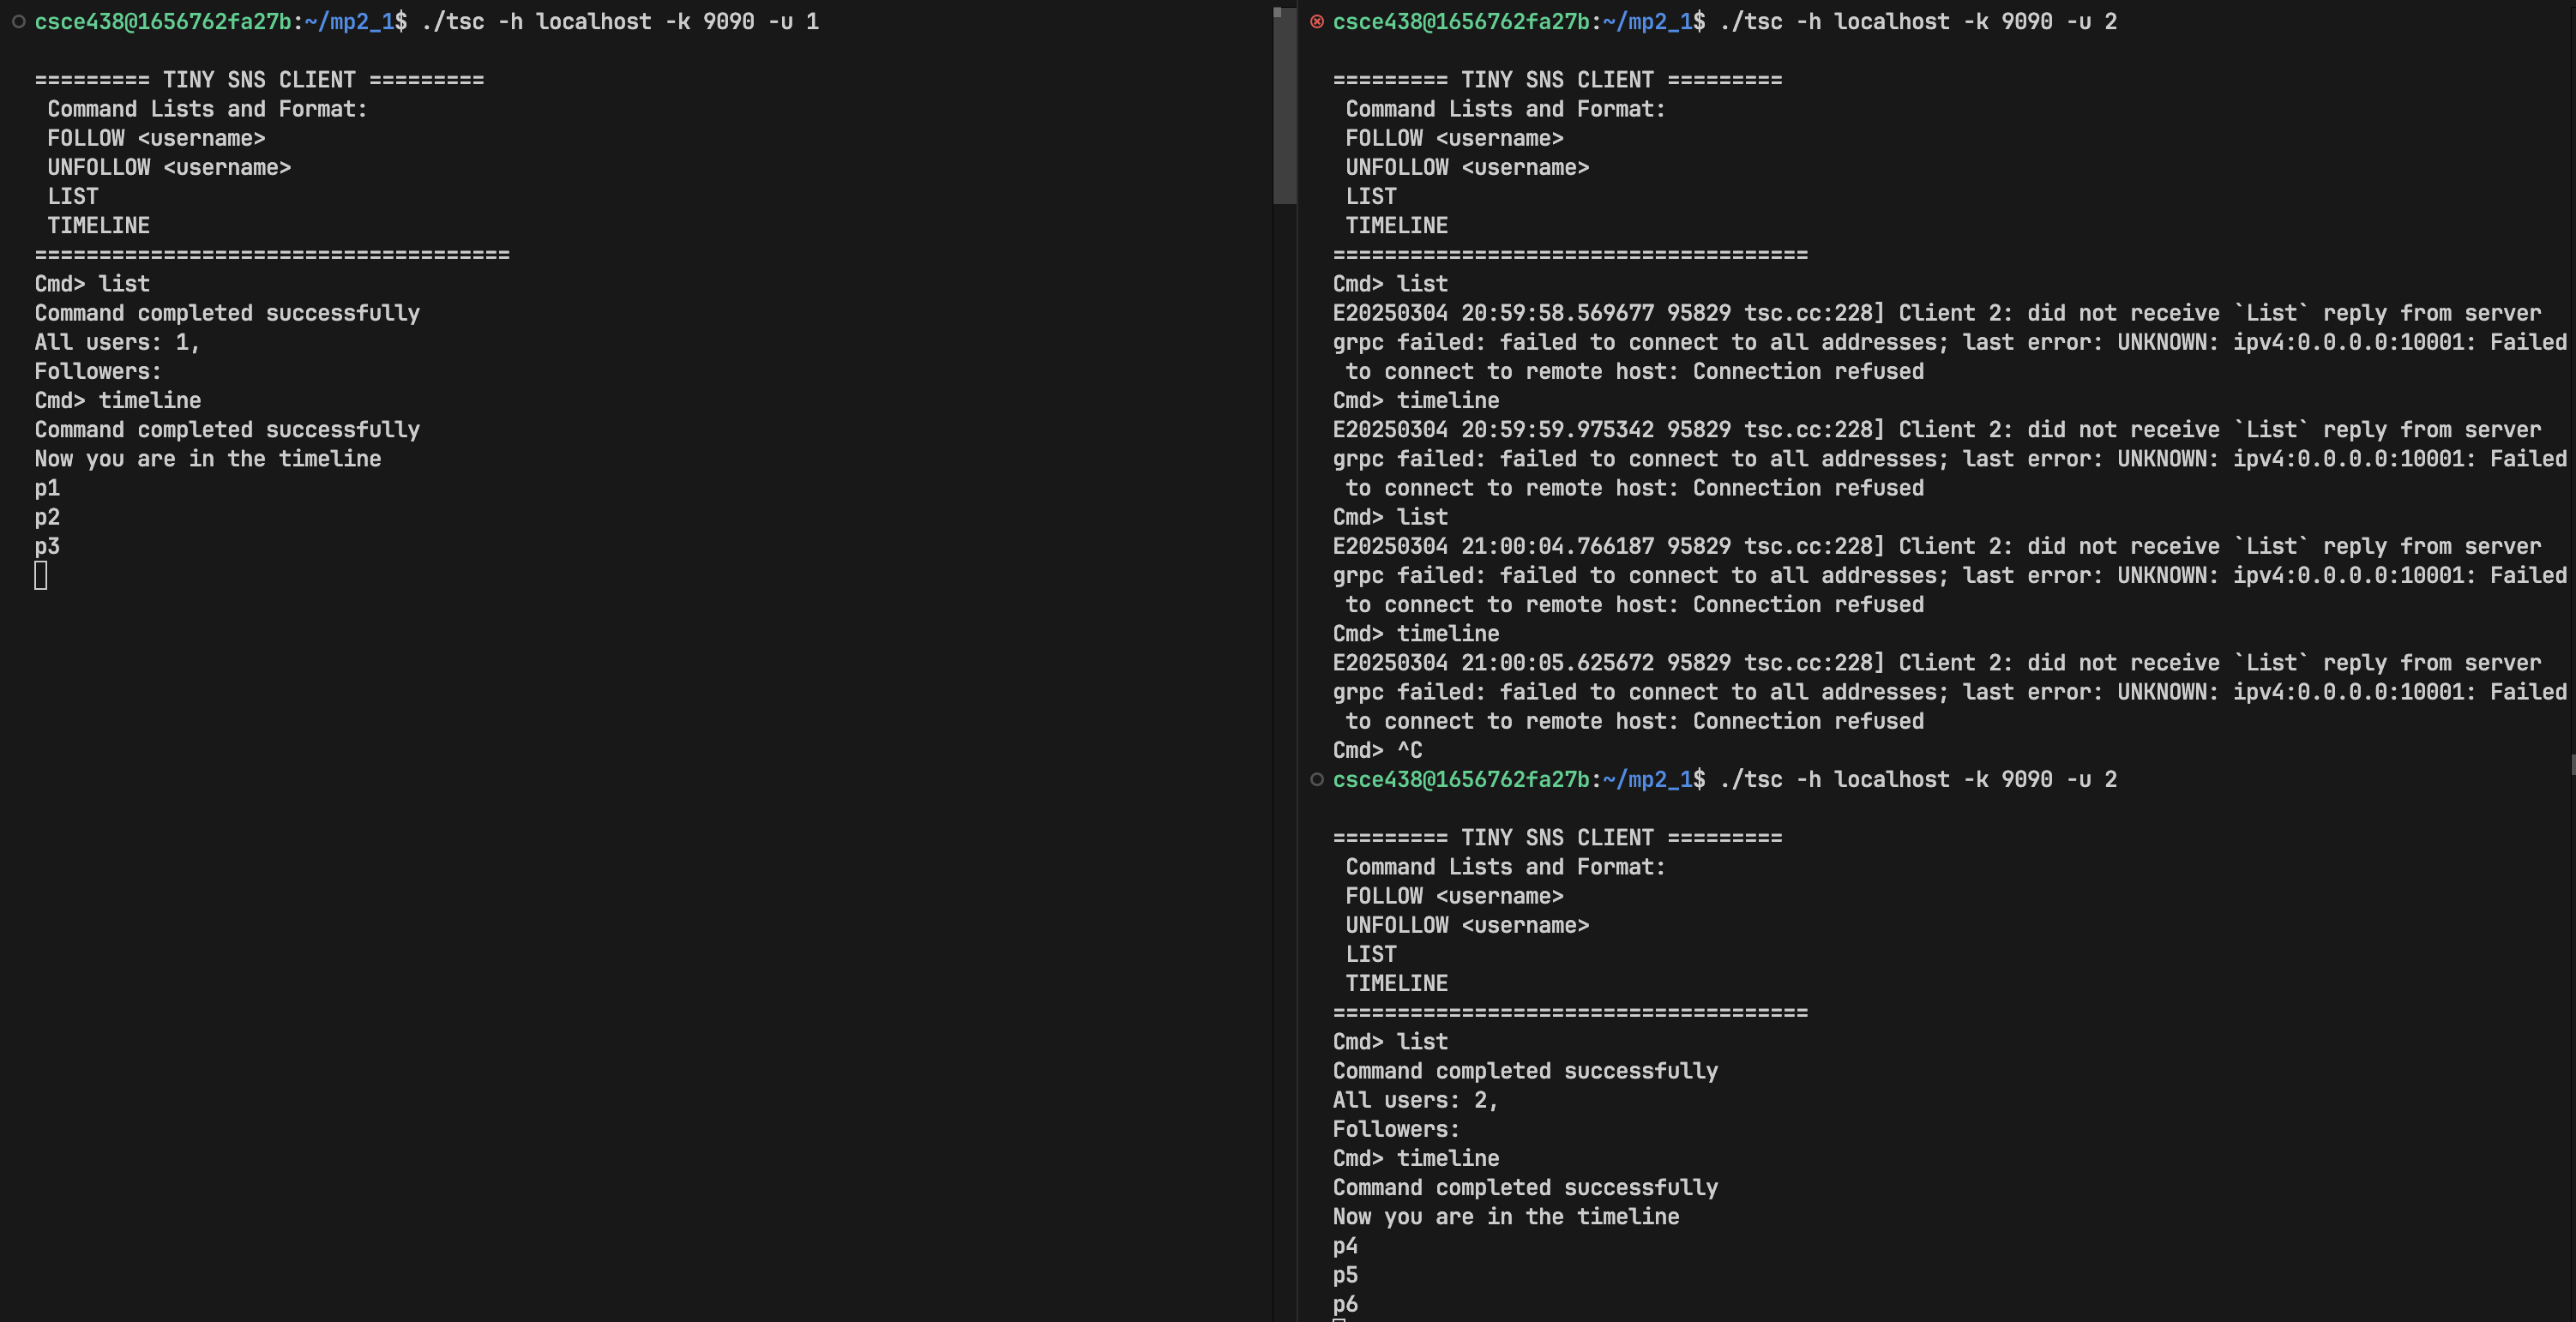
\includegraphics[width=\textwidth]{test3-2}

\end{document}